\documentclass[final]{beamer} % beamer 3.10: do NOT use option hyperref={pdfpagelabels=false} !
% \documentclass[final,hyperref={pdfpagelabels=false}]{beamer} % beamer 3.07: get rid of beamer warnings
\mode<presentation>
{ %% check http://www-i6.informatik.rwth-aachen.de/~dreuw/latexbeamerposter.php for examples
  % \usetheme{Berlin} %% you should define your own theme e.g. for big headlines using your own logos
  \setbeamercovered{transparent} } \usepackage[english]{babel}
\usepackage{caption} \usepackage[latin1]{inputenc}
\usepackage{amsmath,amsthm, amssymb, latexsym} \usepackage{tikz}
\usetikzlibrary{arrows} \usepackage{pgfplots} \usepackage{fix-cm}
% \usepackage{times}\usefonttheme{professionalfonts} % times is obsolete
\usefonttheme[onlymath]{serif} \boldmath
% \usepackage[orientation=portrait,size=a0,scale=1.4,debug]{beamerposter} % e.g. for DIN-A0 poster
% \usepackage[orientation=portrait,size=a1,scale=1.4,grid,debug]{beamerposter} % e.g. for DIN-A1 poster, with optional grid and debug output
\usepackage[size=custom,width=200,height=160,scale=1.4,debug]{beamerposter} % e.g. for custom size poster
% \usepackage[orientation=portrait,size=a0,scale=1.0,printer=rwth-glossy-uv.df]{beamerposter} % e.g. for DIN-A0 poster with rwth-glossy-uv printer check
% ...
\setbeamertemplate{footline}{} \setbeamertemplate{headline}{}
\setbeamertemplate{caption}[numbered] \setbeamertemplate{itemize
  item}{\raisebox{0.23ex}{\large$\blacktriangleright$}\hskip0.1em}
\title[]{{\fontsize{185}{240}\selectfont \textbf{Clustering and
      Diagnosing Patients with Rare Genetic Disorders}}}
\author[]{\huge Jialin Song and Jonathan Zung} \institute[University
of Toronto]{\huge Computational Biology Lab, University of Toronto}
\date{}
\begin{document}
\begin{frame}{}
  \vspace{-2cm}
  \maketitle
  \vspace{-3cm}
  \begin{columns}[T]
    \begin{column}{0.3\linewidth}
      \vbox to 0.82\textheight{
        \begin{block}{\Huge \textbf{Introduction}}
          \Large Rare genetic disorders are caused by abnormalities in
          the human genome. Due to different levels of gene expression
          and influences from the environment, even patients with a
          same underlying disorder may exhibit varying symptoms, which
          makes accurate diagnosis challenging. By taking into account
          statistics on the prevalence of different phenotypes as well
          as the relationships between phenotypes provided by
          ontologies, we can design more informed algorithms for
          analyzing patient data.

    \end{block}
    \vfill
    \begin{block}{\Huge \textbf{Objectives}}
      \begin{itemize}
        \Large
      \item \textbf{Diagnose patients}: We want to help clinicians
        find the correct disorder from among thousands of
        possibilities.
      \item \textbf{Cluster patients with similar phenotypes}: We want
        to present clinicians with similar cases so that knowledge
        about treatment and underlying mechanisms may be shared
        between them.
      \end{itemize}
    \end{block}
    \vfill
   
    \begin{block}{\Huge \textbf{Resources}}
      \begin{block}{\Large \textbf{HPO}}
        \begin{columns}[T]
          \begin{column}{.5\textwidth}
            \centering 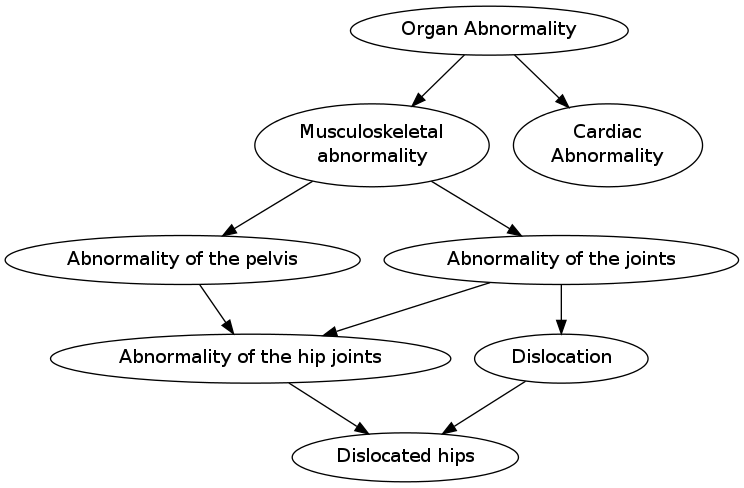
\includegraphics[width = .9\textwidth]{hpo}
          \end{column}
          \begin{column}{.5\textwidth}
            \Large The Human Phenotype Ontology (HPO) organizes
            standardized terms describing abnormal human phenotypes as
            a directed acyclic graph. More specific terms are children
            of more general terms. For example, ``dislocation'' is a
            child of ``abnormality of the joints''.
          \end{column}
        \end{columns}
      \end{block}

      \begin{block}{\Large \textbf{OMIM}}
        \begin{columns}[T]
          \begin{column}{.5\textwidth}
            \centering 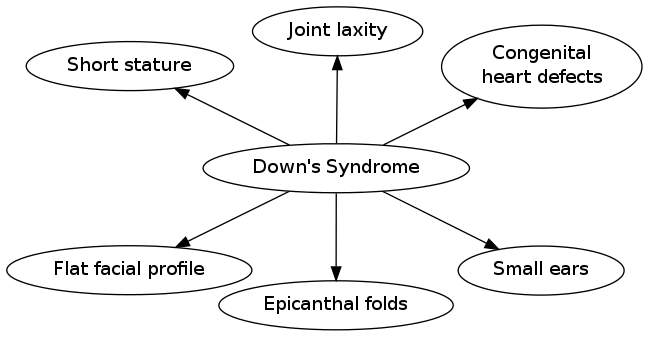
\includegraphics[width =
            .9\textwidth]{omim_vis}
          \end{column}
        
        \begin{column}{.5\textwidth}
          \Large Online Mendelian Inheritance in Man (OMIM) is a large
          database of human genetic disorders. It associates each
          disorder with a list of standard human phenotypes and the
          probabilities with which they occur in patients having the
          disorder. For example, it indicates that a patient with
          Down's syndrome has a probability of 0.5 of having a heart
          defect.
        \end{column}
      \end{columns}
    \end{block}

  

    \begin{block}{\Large \textbf{PhenoTips}}
      \begin{columns}[T]
        \begin{column} {.5\textwidth}
          \centering
          
\includegraphics[width=.9\textwidth]{PhenoTips}
        \end{column}
        
        \begin{column}{.5\textwidth}
          \Large PhenoTips is a web application which helps clinicians
          to record patients' phenotypic profiles using standard HPO
          terms. Standard terminology eliminates ambiguities in
          symptom descriptions.
        \end{column}
      \end{columns}
    \end{block}
  \end{block}
  \vfill
  \begin{block}{\Huge \textbf{Previous Work}}
    \Large Phenomizer (Robinson et al., 2008 {\it{\Large AM J HUM
        GENET 83}}, 610 - 615)

    Phenomizer computes the similarity between two sets of phenotypes
    $S$ and $T$.

    Let $p(t)$ be the probability of a phenotype $t$ in the general
    population.

    The similarity between two phenotypes $s$ and $t$ is defined
    as\[sim(s,t) = \underset{a \text{ a common ancestor of $s$ and
        $t$}}{max} -\log p(a)\]

    The similarity between two sets of phenotypes $S$ and $T$ is
    defined by averaging certain pairwise similarities:
    \[sim(S,T) = avg[\sum\limits_{s \in S} \underset{t \in T}{max}
    sim(s, t) ] + avg[\sum\limits_{t \in T} \underset{s \in S}{max}
    sim(t, s) ] \]

    This method can be applied both to measure the similarity between
    a pair of patients and between a patient and a disorder.
  \end{block}
}
\end{column}

 \begin{column}{0.3\linewidth}
   \vbox to 0.82\textheight{
     \begin{block}{\Huge \textbf{Clustering Methods}}
       \Large
       \begin{block}{\Large \textbf{Patient-Patient similarity
             metrics}}
         We can define a patient-patient similarity metric, and then
         apply a standard clustering algorithm (in our case, spectral
         clustering).

         Examples of similarity metrics:
         \begin{itemize}
         \item Euclidean Metric: Count the number of phenotypes shared
           between two patients.
         \item Information Metric: Here we count shared phenotypes
           weighted by their log probabilities in the general
           population, so that patients sharing rarer phenotypes are
           more similar. The similarities are normalized by the
           analagous weighted count of the total number of phenotypes
           for the two patients.
         \end{itemize}
       \end{block}

       \begin{block}{\Large \textbf{Mixture Models}}
         First we formulate a probabilistic model for patient
         phenotypes with a single latent variable $d$ representing the
         underlying disorder. We can use the EM algorithm to fit the
         model, and then cluster by the inferred values of $d$.

         Examples of mixture models:
         \begin{itemize}
         \item Independent Mixture: Phenotypes are independent given
           $d$.
         \item Conditional Mixture: Phenotypes are conditionally
           independent given $d$ and their ancestors in HPO. In order to
           have a phenotype, a patient must also have its ancestors in
           HPO.  \end{itemize}
       \end{block}
     \end{block}
     \vfill

     \begin{block}{\Huge \textbf{Diagnosis Methods}}
       \begin{block}{\Large \textbf{Naive Bayes}}
         \begin{itemize}
           \Large
         \item For a patient $p$, we want to find the disorder $d$
           with the highest conditional probability $Prob(d \mid p )$.
         \item By Bayes' Theorem,
           \[Prob(d \mid p) = \frac{Prob(p \mid d) \times
             Prob(d)}{Prob(p)} \propto Prob(p \mid d) \times Prob(d)\]
         \item Naive Bayes assumes that each phenotype is independent
           once a disorder is given
           \[Prob(d \mid p) \propto Prob(d) \times \prod_i
           Prob(phenotype_i \mid d)\]
         \end{itemize}
       \end{block}

       \begin{block}{\Large \textbf{Phenotype Matching}}
         \begin{itemize}
           \Large
         \item The objective is to measure how close a patient is to
           the canonical form of a disorder.
         \item For each of a patient's phenotypes, compute the closest
           distance to each phenotype annotation of a
           disorder. Construct a distance matrix from the calculated
           data.
         \item Use the cost matrix to determine the matching between
           patient's phenotypes and disorder annotations that
           minimizes the total distance.
         \item The minimimum distance required to transform from the
           real patient to the canonical form of a disorder is used as
           the measure for closeness.
         \end{itemize}
         \vspace{0.5cm}
         \begin{figure}
           \centering
           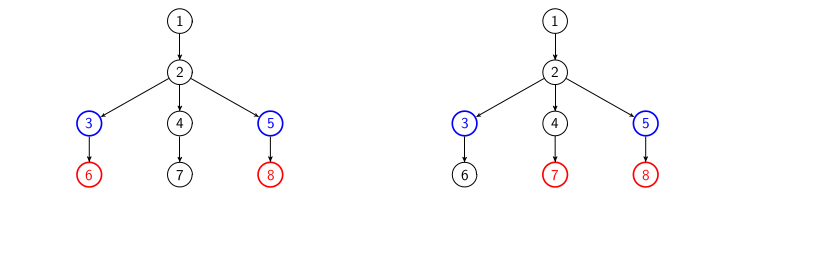
\includegraphics[width=.9\textwidth]{toy_ontology}
           \vspace{0.5cm}
           \caption*{\large A Toy Example}
         \end{figure}
         \Large A patient's phenotypes are marked in blue and the
         annotations of a disorder are marked in red. In the example
         on the right, the real patient can transform into the
         canonical form of a disorder via $3 \rightarrow 2 \rightarrow
         4 \rightarrow 7$ and $5 \rightarrow 8$, resulting in a total
         cost of 4. In the left example, we can achieve a total cost
         of 2 by $3 \rightarrow 6$ and $5 \rightarrow 8$.
       \end{block}
     \end{block}
   }
 \end{column}

 \begin{column}{0.3\linewidth}
   \vbox to 0.82\textheight{
     \begin{block}{\Huge \textbf{Datasets}}
       \Large 25 real patients from published studies
       \begin{itemize}
       \item 13 with Floating Harbor syndrome
       \item 6 with Rubinstein-Taybi syndrome
       \item 6 with Opitz-Kaveggia syndrome
       \end{itemize}
       1498 simulated patients
       \begin{itemize}
       \item A patient is simulated by selecting a disorder at random,
         and then assigning phenotypes to the patient according to the
         probabilities recorded on OMIM. Noise is then added by
         appending some of the 100 most common phenotypes and then
         performing a random walk on the HPO graph.
       \end{itemize}
     \end{block}
     \vfill
     \begin{block}{\Huge \textbf{Clustering Results}}
       \begin{figure}
         \centering
         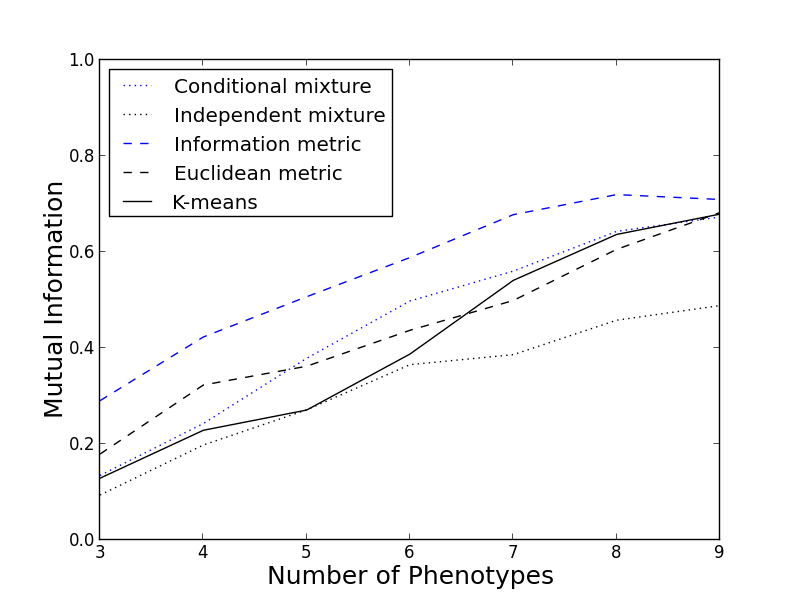
\includegraphics[width=0.6\textwidth]{cluster_comparison.png}
         \vspace{0.5cm}
         \caption*{\large Clustering Results for 25 Real Patients}
       \end{figure}
       \Large The figure above compares clustering results for five
       algorithms on the 25 real patients. To make the clustering
       problem more difficult, the algorithms were only provided with
       a random subset of between 3 and 9 of each patient's
       phenotypes. The vertical axis shows the adjusted mutual
       information of the computed clustering with the true
       clustering.

       The information metric outperformed the Euclidean metric by
       giving rare symptoms more weight. The conditional mixture model
       outperformed the independent mixture model by modelling the
       restriction that a phenotype may only be present when its
       ancestors are.
     \end{block}
     \vfill
     \begin{block}{\Huge \textbf{Diagnosis Results}}
       \begin{figure}
         \centering
         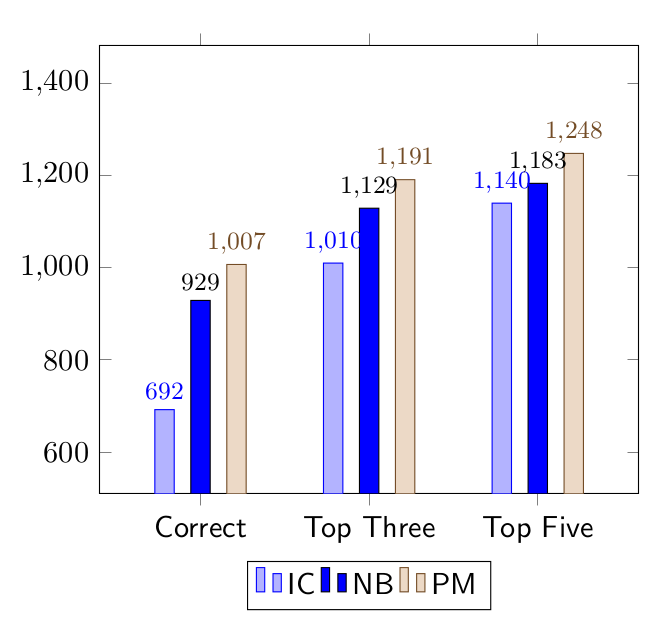
\includegraphics[width=.6\textwidth]{sim_patients}
         \vspace{0.5cm}
         \caption*{\large Diagnosis Results for 1498 Simulated
           Patients}
       \end{figure}
       \Large Naive Bayes made nearly 35\% more correct diagnoses than
       Phenomizer by taking into account the incidence rates of
       abnormal phenotypes, while phenotype matching outperformed
       naive Bayes by utilizing structural information in HPO.

     \end{block}
   }
 \end{column}

\end{columns}
\end{frame}
\end{document}
